%\documentclass[11pt, a4paper]{article}
\documentclass[11pt, a4paper]{scrartcl}

%\usepackage[a4paper,lmargin={3cm},rmargin={3.5cm}, tmargin={2.5cm},bmargin = {2.5cm}]{geometry}
\usepackage{setspace}
\usepackage{indentfirst}
\usepackage{enumitem}
\usepackage{amsmath, amssymb}
\usepackage{graphicx}
\usepackage[backend=biber, authordate, ibidtracker=context]{biblatex-chicago}
\usepackage{fontspec}
\usepackage{titlesec}

\newcommand{\mh}[1]{\noindent\emph{#1}}
\newcommand{\Ssa}{S_{\sigma\alpha}}
\newcommand{\Stsa}{S^t_{\sigma\alpha}}
\newcommand{\sa}{{\sigma\alpha}}
\newcommand{\given}[1][]{\:#1\vert\:}
\newcommand{\Sm}{\Stsa~m^t_{\sa}}
\newcommand{\CI}{\mathrel{\perp\mspace{-10mu}\perp}}
\newcommand{\nCI}{\centernot{\CI}}
\newcommand{\Var}{\mathrm{Var}}
\renewcommand{\i}[1]{\emph{#1}}
\renewcommand{\a}{\alpha}
\renewcommand{\b}[1]{{\osfamily{}#1}}
\newfontfamily\osfamily{Latin Modern Roman Demi}
\setkomafont{disposition}{\osfamily}
\setkomafont{descriptionlabel}{\osfamily}

\onehalfspacing{}
\addbibresource{preemption.bib}
\titleformat{\section}{\Large\bfseries\osfamily}{\thesection}{1em}{}
\titleformat{\subsection}{\large\bfseries\osfamily}{\thesubsection}{1em}{}


\title{\textbf{How to Deal With Expert Testimony} }
\subtitle{The Preemption View in the Olsson-Vallinder Model for Social Networks }
\author{Conrad Friedrich \\ \texttt{conradfriedrich@posteo.net}}
\publishers{Formal Methods II \\ MCMP @ LMU Munich \\ }
\begin{document}

\maketitle
\thispagestyle{empty}
\tableofcontents
\newpage
\section{Introduction}
Is expert testimony just another source of evidence? Or does it have an epistemically special status that should be reflected in how we rationally update our credences? In this paper, I compare two different strategies of dealing with expert testimony, the standard Bayesian way and another, called the Preemption View of authority testimony. To this end I extend the Olsson Vallinder model for social networks to accommodate this recently proposed strategy. Given some plausible assumptions, I surprisingly find that the result do not favor the Preemption View, although of course caveats apply and are addressed.

\subsection{Expert Testimony}
Your doctor examines the red spots on your face and diagnoses: You have the measles! This gives you an excellent reason to believe that you actually have the measles. On the contrary, your accountant concludes that you have lupus does not give you a good reason to believe so.\footnote{This example is from \textcite{Constantin2017}.}

What's the difference? Of course, your doctor knows what she is talking about. She is an \i{expert} in diagnosing patients. What is the reasonable doxastic response to an expert's testimony? This paper examines two different general types of response to a case dubbed Novice/Expert problem \parencite{Goldman2001} for those cases in which the expert is an epistemic authority for the novice, which will be defined below. Note that cases of a novice and multiple experts are \i{not} addressed in this paper, although definitely interesting.\footnote{With a few adaptions, the model could be made to fit those cases, too. As the structure is that of a social network already, it recommends itself for these kinds of questions.}

The first type of doxastic response --- how to update your beliefs in the face of new evidence, in this case expert testimony --- is usually attributed to Thomas Kelly \parencite{Kelly2010-KELPDA} and called the \i{Total Evidence View}. In a rather simplistic rendition relevant to this paper, the view might be summarized as follows: The expert's testimony is added to your stock of evidence for a proposition$p$. It may have a lot of evidential weight compared to the rest of your evidence, since you are competent enough to recognize the expert as an expert. Your own evidence and considerations, however, still bear on the question whether $p$, and are aggregated with the authority's testimony. So far, so standard --- it does not seem like anything else than very standard belief updating. \textcite{Constantin2017}, following \textcite{Zagzebski2012-ZAGEAA} and \textcite{Keren2014-KERTAB}, propose a different strategy called the \i{Preemption View} based on a concept of epistemic authority, which will be discussed next.

\subsection{Epistemic Authority and the Preemption View}

In short, the Preemption View states that in case of authority testimony, you should rationally believe like the authority does, disregarding your own evidence in that matter. In other words, the evidential weight of your own evidence gets reduced to zero in this consideration.

Let's unpack how \textcite{Constantin2017} develop this. First, the testifier has to be judged to be an expert by the agent whose doxastic attitudes are examined. They define, after \textcite{Goldman2001}, someone to be an expert in a certain area of expertise as (a) having a substantial body of evidence and (b) possessing and employing generally truth-conducive methods. Compared to a novice, an expert is an \i{epistemic superior} in her domain of expertise, someone who is more likely to be correct in matters of that domain. Epistemic superiority includes competence in evaluating evidence as well as access to substantive evidence. In particular, evidence that the expert \i{lacks} evidence that the novice possesses licences the novice to withdraw her judgment that the expert is an epistemic superior in this case. 

Now, for an expert $A$ to be an \b{Epistemic Authority} for a novice $N$ in a domain $D$, $N$ has to reasonably believe that 
\begin{enumerate}[label = (\roman*)]
    \item $A$ is an expert about $D$, and
    \item $A$ is epistemically superior to $N$ with respect to $D$.
\end{enumerate}
A domain is a set of propositions best accessible by methods the expert has at her disposal. Note that while it is likely that $A$ is \i{actually} $N$'s epistemic superior, it doesn't necessarily have to the case, since what is crucial here is $N$'s reasonable belief, which can plausibly non-veridic. 

With these preliminaries in place, we can now reconstruct the central claim of \textcite{Constantin2017}. 
\begin{description}
    \item[Preemption View.] An authority's $A$'s testimony that $p$ in $A$'s expertise preempts all evidence of novice $N$ for or against $p$. Evidence is preempted with respect to $p$ if and only the evidence is rationally unusable for $N$ to assess $p$. 
\end{description}

In other words, the evidence is bracketed, so to speak, and loses its evidential force for $p$. It does not lose its evidential weight with respect to all other propositions, though.\footnote{As long as it Preemption View is complemented with another principle of rationality that requires something like consistency, this is not much of a problem. Otherwise it would be easy to find examples where evidential support against $p$ is preempted, but support against an obvious logical consequence of $p$, $q$, isn't, potentially leading to inconsistent belief sets.} 

Let's illustrate with an example from \textcite{Constantin2017}. 

\begin{singlespacing}
\begin{quote}
    Based on observations of everyday occurrences of pairs of events, it appears obvious to a layperson that two events are either simultaneous or they are not. Now she hears that widely respected physicists who specialize in relativity theory believe that this is not true [Such that it's not a fact of the matter whether two events are simultaneous, c.f.]. In this case, it seems completely irrational for the layperson to give any epistemic weight to her own everyday experiences in the face of the verdict of clearly identified experts. She should just follow the authority's lead. 
\end{quote}
\end{singlespacing}

Constantin and Grundmann take this as a case clearly speaking in favor of the Preemption View, based on pre-theoretic judgments and intuitions. They argue for it by presenting the principle as a special case of another normative principle widely accepted. Specifically, preemption works off undercutting defeat. Loosely speaking, some information $d$ is an undercutting defeat for some evidence $e$ towards some proposition $p$ if it removes or weakens the evidential of $e$ for $p$. To give an oft-quoted example of \textcite{Pollock1986}: In a factory, a person looks at an assembly line of widgets that appear red. Being appeared to red-widgetly, the person believes that the widgets are red. But a worker informs the person that there's a red light shining on the widgets, defeating her belief in the color of widgets, making it irrational to hold in the light of the defeater. Preemption, then, is a result from this type of defeat: The authority's testimony undercuts the rationality of trusting your own evidence. Here lies the argument for Constantin and Grundmann's normative claim.

\subsection{The Need for Precisification}

While the account is promising and well-argued for in the case for flat-out, or ternary, belief, it is much less fine-tuned if you take a look at what this means for degrees of belief as a framework of doxastic states. Especially the main argument is worrisome: To my knowledge, there hasn't been a worked-out theory of undercutting defeat for degrees of belief so far. At least Constantin and Grundmann are not mentioning one. The result is that in the case of degree of belief, it is rather unclear what the conditions are for authorities to be recognized as such, or for reasons to be preempted. Worse, without a general principle of undercutting defeat to defer to, the normativity of the preemption principle stands questioned. This is not \i{necessarily} bad news for their account, as the problems do not arise for flat-out belief. But since they explicitly state to include degrees of belief in their argument, it is worth to have a closer look. 

This is not the place to to give an attempt at a general account of undercutting defeat. Instead, I want to argue from a different angle: Given some plausible ways to translate the Preemption View into a precise computer model, and assume a veritist position from which to argue for the normativity of a principle, as described in the next section. But as it turns out, the experiment setup is this paper does not yield a corroborating result for the Preemption View. 

\subsection{Evaluation}

What kind of argument can the present paper deliver? In brief, it strives to be a normative one, of course, since the question which rational strategy to employ is a strictly normative one. The ground for this normative claim are teleological: veritist epistemology assumes truth to be a fundamental epistemic value, and since truth-directed strategies promote this value, they should be followed. This consequentialist picture is, of course, not without substantial debate,\footnote{cf. \textcite{Goldman2001} for an argument for a veritistic approach to epistemic normativity. A very readable argument against is presented in \textcite{Berker2013}.} this is philosophy after all, but the present paper is not the place to discuss this (albeit interesting) issue. The veritist account, of course, lends itself quite ideally to formal treatment, as it gives the researcher tools and methods to quantify the epistemic value of doxastic attitudes and with a consequentialist approach to normativity derive normative claims. 

\section{Model Description}

The Model used in this paper follows the one proposed by \textcite{Olsson2013} rather closely. I adopt most of their formalizations and assumptions. To enable the reader to make use of the derivations in \textcite{Angere2010}, I adopt their notations as well. I summarize the model, describe how I use it for the present purposes and make note of any deviation.

The core entities of the model are \i{agents} and their properties. Agents can be connected to one another, such that they form a network. Since these connections enable communication and the agents are meant to represent people, this structure can be seen as a social network, represented in some form of graph representation through an adjacency matrix.

The model has certain starting parameters, which I describe below, and discrete time steps. Each of these enable the update of properties by the rules specified further below.

\subsection{Starting Parameters}

To keep things manageable, there is a single \i{true} target proposition $p$ which the agents have a credence $C^t_\alpha(p)$ towards. Each time step, agents can receive information from a \i{source}. These can be (i) other agents in the social network or (ii) their own inquiry. The objective chance that an agents inquires and gets it right is called that agent $\alpha$'s \i{aptitude}: $P(S_{\iota \alpha}p \given S_{\iota \alpha} \land p)$, where $S_{\iota \alpha}$ is the chance that agent $\alpha$ inquires for evidence, regardless of the results, and $S_{\iota \alpha} p$ the chance that she inquires and her inquiry yields $p$ as a result. The chance that she inquires at all, $P(S_{\iota \alpha})$, is called her \i{activity}. For the sake of simplicity, these chances are modeled as time invariant.

Sources can be more or less reliable. The reliability is assumed to be symmetric.
\[ 
R_{\sigma \alpha} =_{df.} P(\Ssa p \given \Ssa \land p) = P(\Ssa \neg p \given \Ssa \land \neg p)
\]
This is, of course, just the agent's aptitude. Note that the reliability of an agent is modeled continuously, in contrast to the binary full reliability/randomiser approach employed in \textcite[Chp. 3]{Bovens2003}, such that with a reliability value of less than $.5$ an agents inquiry would actually be negatively correlated with the truth.

Each agent trusts each source to a certain extent. This is expressed in the agent's credence in the reliability of the source:
\[ 
    C^t_{\alpha}(a \leqslant R_{\sa} \leqslant b) = \int_a^b \tau^t_{\sa}(\rho) d\rho
\]
where $\tau^t_{\sa}: [0,1] \rightarrow \mathbb{R}^+$ is a probability density function such that 
\[
    C^t_{\alpha}(0 \leqslant R_{\sa} \leqslant 1) =  \int_0^1 \tau^t_{\sa} (\rho) d\rho = 1
\]which is a very plausible requirement on a rational credence function.\footnote{In fact, not obeying this would violate the probability axioms. For some reason, \textcite{Angere2010} as well as \textcite{Olsson2013} define the trust function as $\tau^t_{\sa}: [0,1] \rightarrow [0,1]$, such that it doesn't integrate to 1 (in all but the trivial case). I assume they are doing some hidden normalising that I am to near-sighted to see.}

\begin{description}
    \item[Example.] An agent $\alpha$ with a healthy trust in her own inquisitive abilities and who is not easily swayed in this trust may have a trust function $\tau^t_{\iota\alpha}$ described by a beta distribution
\[
    \tau^t_{\iota\alpha} (\rho) = \frac{1}{B(a,b)} \rho^{a - 1} {(1 - \rho)}^{b-1}
\]
with normalising beta function $B(a,b)$ and parameters $a, b$ chosen such that $\tau^t_{\iota\alpha}$ is densest around whatever a `healthy trust' amounts to, let's say 0.85 (cf.~Fig.~\ref{fig:trf}). Interestingly, the shape of the curve correlates with how resilient the function behaves upon updating. More on that below.
\end{description}

\begin{figure}[ht]
	\centering
    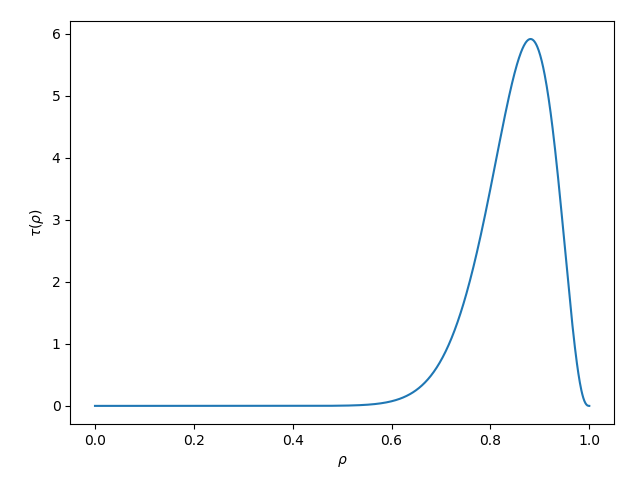
\includegraphics[width=0.5\textwidth]{Figure_1.png}
	\caption{Beta distributed trust function with parameters $a~=~20.825$ and $b~=~3.675$\label{fig:trf}}
\end{figure}

Apart from inquiries, a source can also be another agent, through testimony. An agent $\alpha$ therefore trusts herself at time $t$ with $\tau^t_{\iota\alpha}$ and another agent $\beta$ with $\tau^t_{\beta\alpha}$.

The exchange of information and the evolution of the trust functions and the credences in $p$ are the most important going-ons in this model, which I'll summarize next.

\subsection{Inquiry and Communication} 

Time progress is modeled in discrete steps. At each time step, each agent updates her credence and her trust function. The new information which motivates these changes are messages from the sources, which the agent receives if
\begin{enumerate}[label = (\roman*)]
    \item the agent inquires herself with probability $P(S_{\iota\alpha})$. The result of the inquiry is determined by the agent's aptitude. Or,
    \item another agent $\beta$ is connected to agent $\alpha$ through the social network and decides to share her opinion. This is modeled, in slight deviation from the Olsson-Vallinder model, by the following conditions: 
        \begin{enumerate}[label = (\alph*)]
            \item Agent $\beta$ is sufficiently confident in $p$ resp. $\neg p$, determined by some fairly high threshold value for her credence, and
            \item agent $\beta$ received herself new information in the same time step. In the current implementation, this is only fulfilled by own inquiry.  
        \end{enumerate}
\end{enumerate}

Testimony is, of course, a matter of language, and is most plausibly modeled as a binary judgment, that is, either $p$ or $\neg p$. While there are certainly interesting cases where the testimony involves credences or levels of confidences, e.g. \ a weather forecaster stating her belief in the chance of rain tomorrow, this does in my view not apply to  

\subsection{General Updating}

Each time step, the agents update their credences and trust functions. Updating the credences is based on new messages the agent received this time step: $\Stsa m^t_{\sa}$, where $m^t_{\sa}$ is the message that $\alpha$ received from $\sigma$ (which can represent $\alpha$'s own inquiry or another agent's testimony) at $t$, and is either $p$ or $\neg p$. An agents can receive multiple messages per time step, but only one message per source, so we have to account for that as well. 

In the central and most important deviation from the Olsson Vallinder model, I distinguish between the \i{Preemption} strategy and the \i{Total Evidence} strategy of dealing with expert testimony. In normal circumstances, both strategies involve the same standard bayesian updating rules, which I give in detail below. In the face of expert testimony they may differ, however, and I describe the requirements for differences as well as the differences themselves subsequently. 

The updating rule is given by conditionalisation:
\[
    C^{t+1}_\alpha (p) = C^t_\alpha (p \given \bigwedge_{\sigma \in \Sigma^t_\alpha} \Stsa m^t_{\sa}),
\]

where $\Sigma^t_\alpha$ is the set of sources that send a message to $\alpha$ at $t$.

With the assumption that sources are independent given the target proposition, the update calculates to
\begin{equation}
    \label{eq:upd}
    C^t_\a (p \given \bigwedge \Sm) = \\
     \frac{C^t_\a (p) \prod C^t_\a (\Sm \given p) }
    {C^t_\a (p) \prod C^t_\a (\Sm \given p) +  C^t_\a (\neg p) \prod C^t_\a (\Sm \given \neg p) }.
\end{equation}

Here, again, the product and big conjunct range over all sources with a message for the agent, the subscript omitted for legibility.   

The expressions about the reliability are given by:
\begin{align*}
    C^t_\a (\Stsa p \given p) &= C^t_\a (\Stsa) \langle \tau^t_{\sa} \rangle \\
    C^t_\a (\Stsa \neg p \given p) &= C^t_\a (\Stsa) \langle \bar{\tau}^t_{\sa} \rangle \\
    C^t_\a (\Stsa p \given \neg p) &= C^t_\a (\Stsa) \langle \bar{\tau}^t_{\sa} \rangle \\
    C^t_\a (\Stsa \neg p \given \neg p) &= C^t_\a (\Stsa) \langle \tau^t_{\sa} \rangle,
\end{align*}

where $\langle \tau^t_{\sa} \rangle $ is the expected value of trust function $ \tau^t_{\sa} $ and ${\langle \bar{\tau}^t_{\sa} \rangle =_{df.} 1 - \langle \tau^t_{\sa} \rangle}$.\footnote{Detailed and very helpful derivations of these equations can be found in \textcite{Angere2010}, although in places I could not agree with the results. I implemented the updating mechanism as presented in this paper. There is not much room to detail the finer points here, only this much: Angere's final result on page 22 for the credence update intuitively can't be right, since the expression as stated there does not depend on the actual content of the message, that is, $p$ or $\neg p$, anymore, and instead just updates regardless, rendering the network communication ineffective.} 

Upon receiving a message, the agent updates her trust function for that source depending on how well the message coheres with her own credence. The updated trust function can be calculated to
\[
    \tau^{t+1}_\sa = \tau^t_\sa (\rho) \frac{\rho \: C^t_\a (p) + (1 - \rho) C^t_\a (\neg p)}
    {\langle \tau^t_\sa \rangle C^t_\a(p) + \langle \bar{\tau}^t_\sa \rangle C^t_\a(\neg p)}
\]
if $m^t_{\sa} = p$, and 
\[
    \tau^{t+1}_\sa = \tau^t_\sa (\rho) \frac{\rho \: C^t_\a (\neg p) + (1 - \rho) C^t_\a (p)}
    {\langle \tau^t_\sa \rangle C^t_\a(\neg p) + \langle \bar{\tau}^t_\sa \rangle C^t_\a(p)}
\]
if $m^t_{\sa} = \neg p$. This entails that the trust an agents brings towards a source only changes with regard to the agents credence in p and the source's message whether p. This is one of the major shortcomings of the model, in my view, especially for the current purposes, as at no stage something like higher order evidence about the reliability of the source comes into play. 

\subsection{Updating With Preemption}

In certain cases, an agent who pursues the preemptive strategy differs in her updating rule from what is described above, namely when she recognizes another agent as an epistemic authority. I modeled the requirements in \textcite[p.9]{Constantin2017} for the recognition of an epistemic authority in the following way. 
\begin{description} 
    \item[Epistemic Authority] An agent $\alpha$ recognizes another agent $\beta$ as an epistemic authority regarding proposition $p$ at time $t$ if and only if  
    \begin{enumerate}[label= (\roman*)]
        \item $\langle \tau^t_{\beta\alpha} \rangle \geqslant T_A$, where $T_A$ is a reasonably high threshold of trust, and
        \item $\langle \tau^t_{\beta\alpha} \rangle - \langle \tau^t_{\iota\alpha} \rangle \geqslant \Delta_A$, where $\Delta_A$ denotes a significant difference in trust level.
    \end{enumerate}


\end{description}
    In plain English: Consider a layperson and an expert. For the layperson to regard the expert as an epistemic authority, she has to (i) regard the expert with a high amount of trust. The threshold is high, somewhere above $.8$. Condition (ii) requires that the expert enjoys a significantly higher trust from the layperson than the layperson trusts her own abilities to evaluate evidence. This might also be modeled as a ratio, but in this case is not crucial.

As soon as an agent recognizes another as an epistemic authority, her updating pattern changes significantly. First, she stops to gather evidence herself completely. Second, instead of updating according to all her evidence and sources, she ignores all other messages and instead adopts the authority's opinion.

Constantin and Grundmann do not specify a precise credence as a proper response in this case, as they assume that the layperson knows of the expert's credence. In this model, however, communication happens on a binary basis.
 
I argue that the right credence for the layperson to adopt in this case is just $\langle \tau^t_{\beta\alpha} \rangle$ (if the message is $p$, or $1 - \langle \tau^t_{\beta\alpha} \rangle$ if $\neg p$, the case is an exact analogous). While it is intuitively appealing, it's also a consequence from some rather innocuous assumptions. The argument goes as follows. 

\textcite[p.12]{Constantin2017} define the effect of preemption as making any evidence for or against the target proposition rationally unusable for the agent. That is, whatever first-order evidence she gathered beforehand, as soon as she recognizes an epistemic authority as such regarding that proposition, two things happen: 

First, she is rationally required to disregard all her evidence. It is quite uncontroversial to regard a credence around $.5$ to be rational in the case of total absence of evidence (extreme subjective Bayesians excluded). But being indifferent is certainly not a bad thing in this case. Formally, this can be described as a screening-off. Let $\beta$ be an authority for $\alpha$. Then $\a$'s evidence is preempted by $S_{\beta\a}$ iff for all (relevant) evidence $E$, 
\[ 
    p \CI_{C_\a} E \given S_{\beta\a}, 
\]
that is, relative to $\a$'s credence function, $p$ is independent of $E$ given $S_{\beta\a}$. That is, the rational requirement the authority's testimony induces on the preemption strategist's credences.

Second, the only available evidence is the authority's testimony. The agent classically conditions on that. Given the above, this is calculated quickly. Equation~\ref{eq:upd} reduces in this case to 

\[
    C^{t+1}_\a (p) = \frac{C^t_\a(p) \langle \tau^t_{\beta\a} \rangle}
    {C^t_\a(p) \langle \tau^t_{\beta\a} \rangle + C^t_\a(\neg p) \langle \bar{\tau}^t_{\beta\a} \rangle}
\]
and because I require as mentioned $C^t_\a(p) = C^t_\a( \neg p)$, simple algebra gives 
\[
    C^{t+1}_\a (p) = \langle \tau^t_{\beta\a} \rangle.
\]

The trust functions update in the usual way. They are \i{not} affected by the preemption. This is, in my opinion, actually a strong suit of the model. \textcite[p. XX]{Constantin2017} describe a range of cases in which the purported authority make an  \i{outrageous} claim which is so obviously wrong that the agent should lessen her trust in the authority and do not regard her as such anymore. This is reflected in the model: If the agents beliefs something to an extremely high degree, and a purported authority says otherwise, it is possible to lower the trust in the authority and thereby make her lose her status as an authority for the agent. 

\subsection{Epistemic Value}

To evaluate the epistemic situation of the agents and make an actual normative judgment about which of the strategies if preferable, I adopt a veritistic position and assume that there is some epistemic merit to hold credences with a higher accuracy, that is, a higher closeness to the truth. But I think the veritistic approach makes for a nice framework to evaluate belief states in. 

How to measure epistemic value? In recent literature, the \i{Brier Score} as a quadratic scoring rule has been widely used. Of course, this is philosophy, and it's feasibility is again a contested topic\footnote{cf. \textcite{Joyce1998-JOYANV}, \textcite{Maher2002-MAHJAF} and \textcite{Fallis2016} for a discussion.}, but in the present case there are only credences in a single proposition to evaluate, such that the differences aren't as pronounced. Let's define scores in the following way:
\begin{equation*}
    I_{BR}(C^t_\a) = {(\nu(p) - C^t_\a(p))}^2
\end{equation*}
where $\nu$ is the vindication function that assigns truth values ($\{0,1\}$) to propositions (at the actual world).
A credence function $C^t_\beta$ is then epistemically more valuable than another $C^t_\gamma$ at $t$ if and only if $C^t_\beta(p) < C^t_\gamma(p)$, provided that $p$ exhausts all propositions considered. The brier score hence measures \i{inaccuracy}.

\section{Experiment}

To approach the central question of the paper I set up the experiment minimally. This just consists in three agents, set up like in Fig.~\ref{fig:el}. The edges represent available directions of communication. Additionally, each agent can inquire for herself. Experts and laypersons are modeled by different aptitudes. I refer to the expert as $\varepsilon$, the layperson employing a preemption strategy as $\beta$ and the layperson employing the classical bayesian strategy as $\a$. 

\begin{figure}[ht]
	\centering
    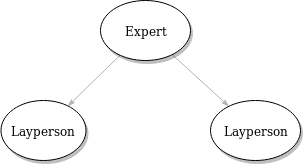
\includegraphics[width=0.5\textwidth]{Expert_Layperson.png}
	\caption{The minimalist setup of the present experiment with an expert and two laypersons employing different updating strategies.\label{fig:el}}
\end{figure}

\subsection{Setup}
The expert is much more likely to inquire correctly than the layperson is, this experiment uses values of $R_{\iota\varepsilon} = 0.85$ and $R_{\iota\a} = R_{\iota\beta} = 0.5$.

In each trial, both credences of the laypersons are set to the same uniformly distributed value. The experts initial credence is given by a beta-shaped meta distribution with a mean of $ 0.85$, meaning that on average over all trials the expert's initial credence is about that value.

The expert's trust in her own inquiry is set quite high, modeled here as a beta distribution with $\langle \tau^0_{\iota\varepsilon} \rangle = 0.85$ and a low $\sigma^2 = 0.005$, indicating that the expert isn't easily influenced in her trust in herself.

The laypersons are slightly overconfident, but more easily swayed, modeled as $\langle \tau^0_{\iota\a} \rangle =\langle \tau^0_{\iota\beta} \rangle = 0.55$ and $\sigma^2 = 0.01$.

The initial values $\langle \tau^0_{\varepsilon\a} \rangle =\langle \tau^0_{\varepsilon\beta} \rangle = 0.8$ with $\sigma^2 = 0.01$ are already quite high.

The assertion threshold, the threshold $T_A$ to recognize an authority and $\Delta_A$ have been set to $0.8, 0.82$ and $0.1$, respectively.

\subsection{Running the Experiment}

A single run of the experiment goes through the updating procedure for each agent as described above, through 10 discrete time steps. All changes in credence are recorded. For a snapshot of a single run of the program, see Fig.~\ref{fig:run} on page~\pageref{fig:run}.

\begin{figure}
	\centering
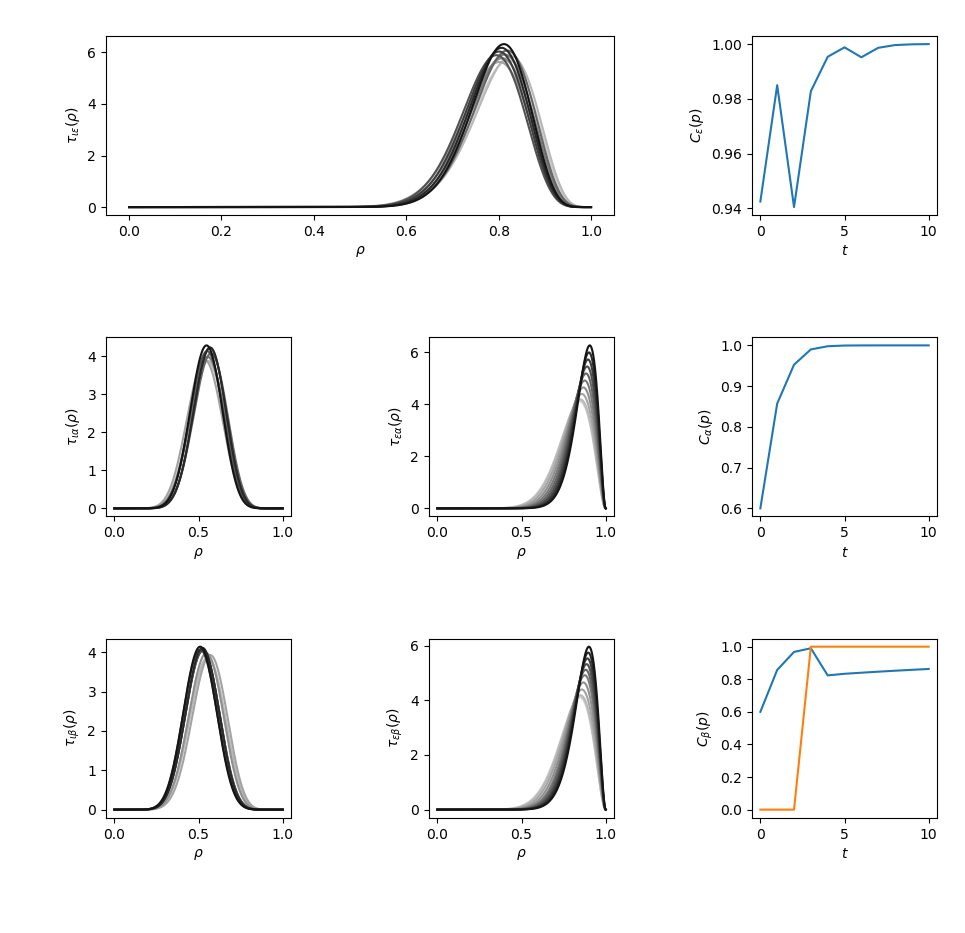
\includegraphics[width=\textwidth]{Run.png}
\caption{Example single run of the experiment with a layperson initial credence of $0.6$. The first row shows the expert's trust function in her own inquiry and her credence, the second row shows the Bayesianist's trust functions in herself and the expert as well as her credence. The third row shows the preemption strategist's trust functions and her credence. The orange line in the bottom right plot indicates whether she recognizes the expert as an authority (1 corresponds to yes). The increasing saturation of the black indicates time progress, the darker plots are later.\label{fig:run}}
\end{figure}

The experiment executes 10000 such runs, varying the starting conditions as described.

\section{Results}

\begin{figure}
	\centering
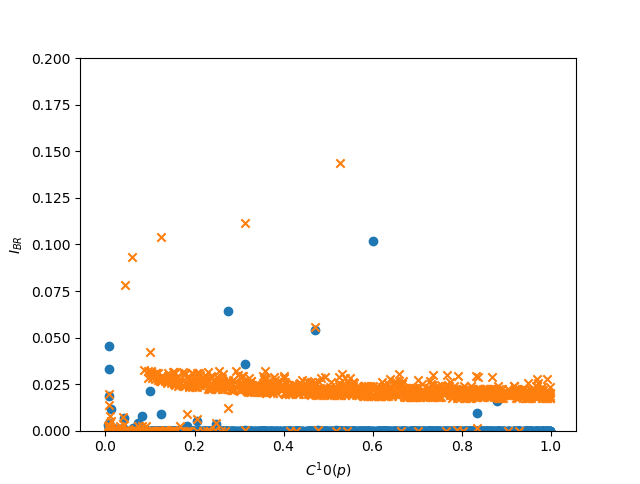
\includegraphics[width=0.8\textwidth]{Result.png}
\caption{Scatter plot of the result of (for legibility only) 1000 runs with the preemption strategist as orange X-markers. It seems that the starting credence has little effect on the Brier score after 10 steps, except for $C^{10} < 0.1$. In these cases, though, it is likely that the agent did not accept the expert as an authority.\label{fig:res}}
\end{figure}

Fig.~\ref{fig:res} gives a scatter plot of the results at $t=10$. After 10000 runs, the average Brier score of the preemption strategist was $\sim0.0254$, compared to the Bayesian's $\sim0.0076$, a stunning difference. An intuitive explanation for this result can be found by a look at Fig.~\ref{fig:run}, bottom right. Agent $\beta$ starts out Bayesian and quickly reaches a credence close to 1. Accordingly, her trust in the expert rises. As soon as the authority-threshold is reached, she drops her credence to $\langle \tau^0_{\varepsilon\a} \rangle $, then continuing to adapt her credence to the trust level. This procedure is a lot slower to approach 1 than the Bayesian, such that after 10 steps the Brier score is higher. Note how the agent's own inquiries do not have any visible effect on the credence at all, mostly due to the low trust level the laypersons have towards there own inquiries.

What does this result suggest? Given all the assumptions that were made are actually accurate, this results speaks against respecting Preemption and recommends instead to update like classically Bayesian. There is no evidence from a veritist standpoint to favor the Preemption view, this much is correct. Is the Total Evidence View correct for credences, after all? The big qualifier at the beginning of this paragraph should give it away: This can only be a small indicator amongst many. Most of the assumptions probably aren't correct. Given time and space constraints, I was not able to explore the parameter space further. Additional research could show that the starting conditions are merely a special case in which the Preemption view isn't as truth-directed, but in other cases, it is. Furthermore, there are different interpretations to what the preemptive updating rule should amount to. More on that and other caveats to this result in the next section.
\newpage
\section{Caveats, Objections and Where to Go From Here}

Unsurprisingly, the proponent of the Preemption View has lots of metaphorical arrows in her quiver to shoot holes in this paper's result. I'll go through them one by one.

First, it may be the case that Constantin and Grundmann don't intend to have this principle apply to degrees of belief as probability functions, they never explicitly state so. There are other possibilities to talk about credences, after all. But since using the probability framework seems very desirable, it would be too boring a cop-out.

Second, as noted before, the model might be to simplistic: it does not respect higher-order-evidence \i{other} for or against trusting an authority than originating directly from the target proposition $p$ through the update of the trust function. But such evidence would be plausible, of course: It is a central tenet of the account to grant the ability to gather second-order evidence and denouncing an epistemic authority when the trust level drops. At present, the model only incorporates this by the comparison of credences in the target proposition $p$. Hence, the recognizing of an expert as an authority is very heavily idealised in the model.

Third, the argument Constantin and Grundmann put forward is supposed to provide a local, immediate strategy, as the examples unanimously speak of few time steps. There is no focus on ``the long run'', if you will, like this model assumes. Perhaps, one could argue, agent based models aren't the best fit then, as they shine once the complexity of a model surpasses analytic tractability. But then, if the strategies are any good, they should survive the test in the long run as well. It'd definitely be worthwhile do examine shorter time frames, too.   

Fourth, the present experiment as designed above does not include the trust function itself in the parameter space of the model. Variating the initial trust function could have significant impact on model behaviour, but due to time constraints, aren't included in the present experiments. A very quick rundown of why that matters: The initial shape of the curve of the trust function heavily affects the expected value's disposition to change after a time step.\footnote{cf. \textcite{Angere2010}.} The narrower the initial distribution is, the less responsive it is to change, given the same parameters of credence and source message.

\begin{itemize}


    \item the starting trust functions are kind of arbitrarily set and may influence the results. Should be put in parameter space and explored! especially the shape of the curve. Or even other functions normalized to integrate to one?
    \item The issue with repeated testimony of the same source regarded as independent
    \item Method of communication can be explored.
\end{itemize}

\printbibliography{}
\end{document}

